%%%%%%%%%%%%%%%%%%%%%%%%%%%%%%%%%%%%%%%%%%%%%%%%%%%%%%%%%%%%%%%%%%
\section{Introduction}\label{intro}

% Why are we studying this problem
Earthquakes can cause great damage to human society through soil
rupture, movement, tsunami, etc. Some recent earthquakes that
highlight this destructive potential are the great East Japan
Earthquake of 2011 (Figure~\ref{GreatEastJapan}), and the
April 2015 earthquake in Nepal. One important tool for the enactment
of policies that minimize the consequences of these events are
earthquake occurrence models (also called risk models). These models
can be used to identify patterns in the seismic mechanisms that
generate earthquakes, and are important to increase our understanding
of these events.


% \cite{ecta14} opening image. Would be better to have a clustered one.
\begin{figure}[]
\centering
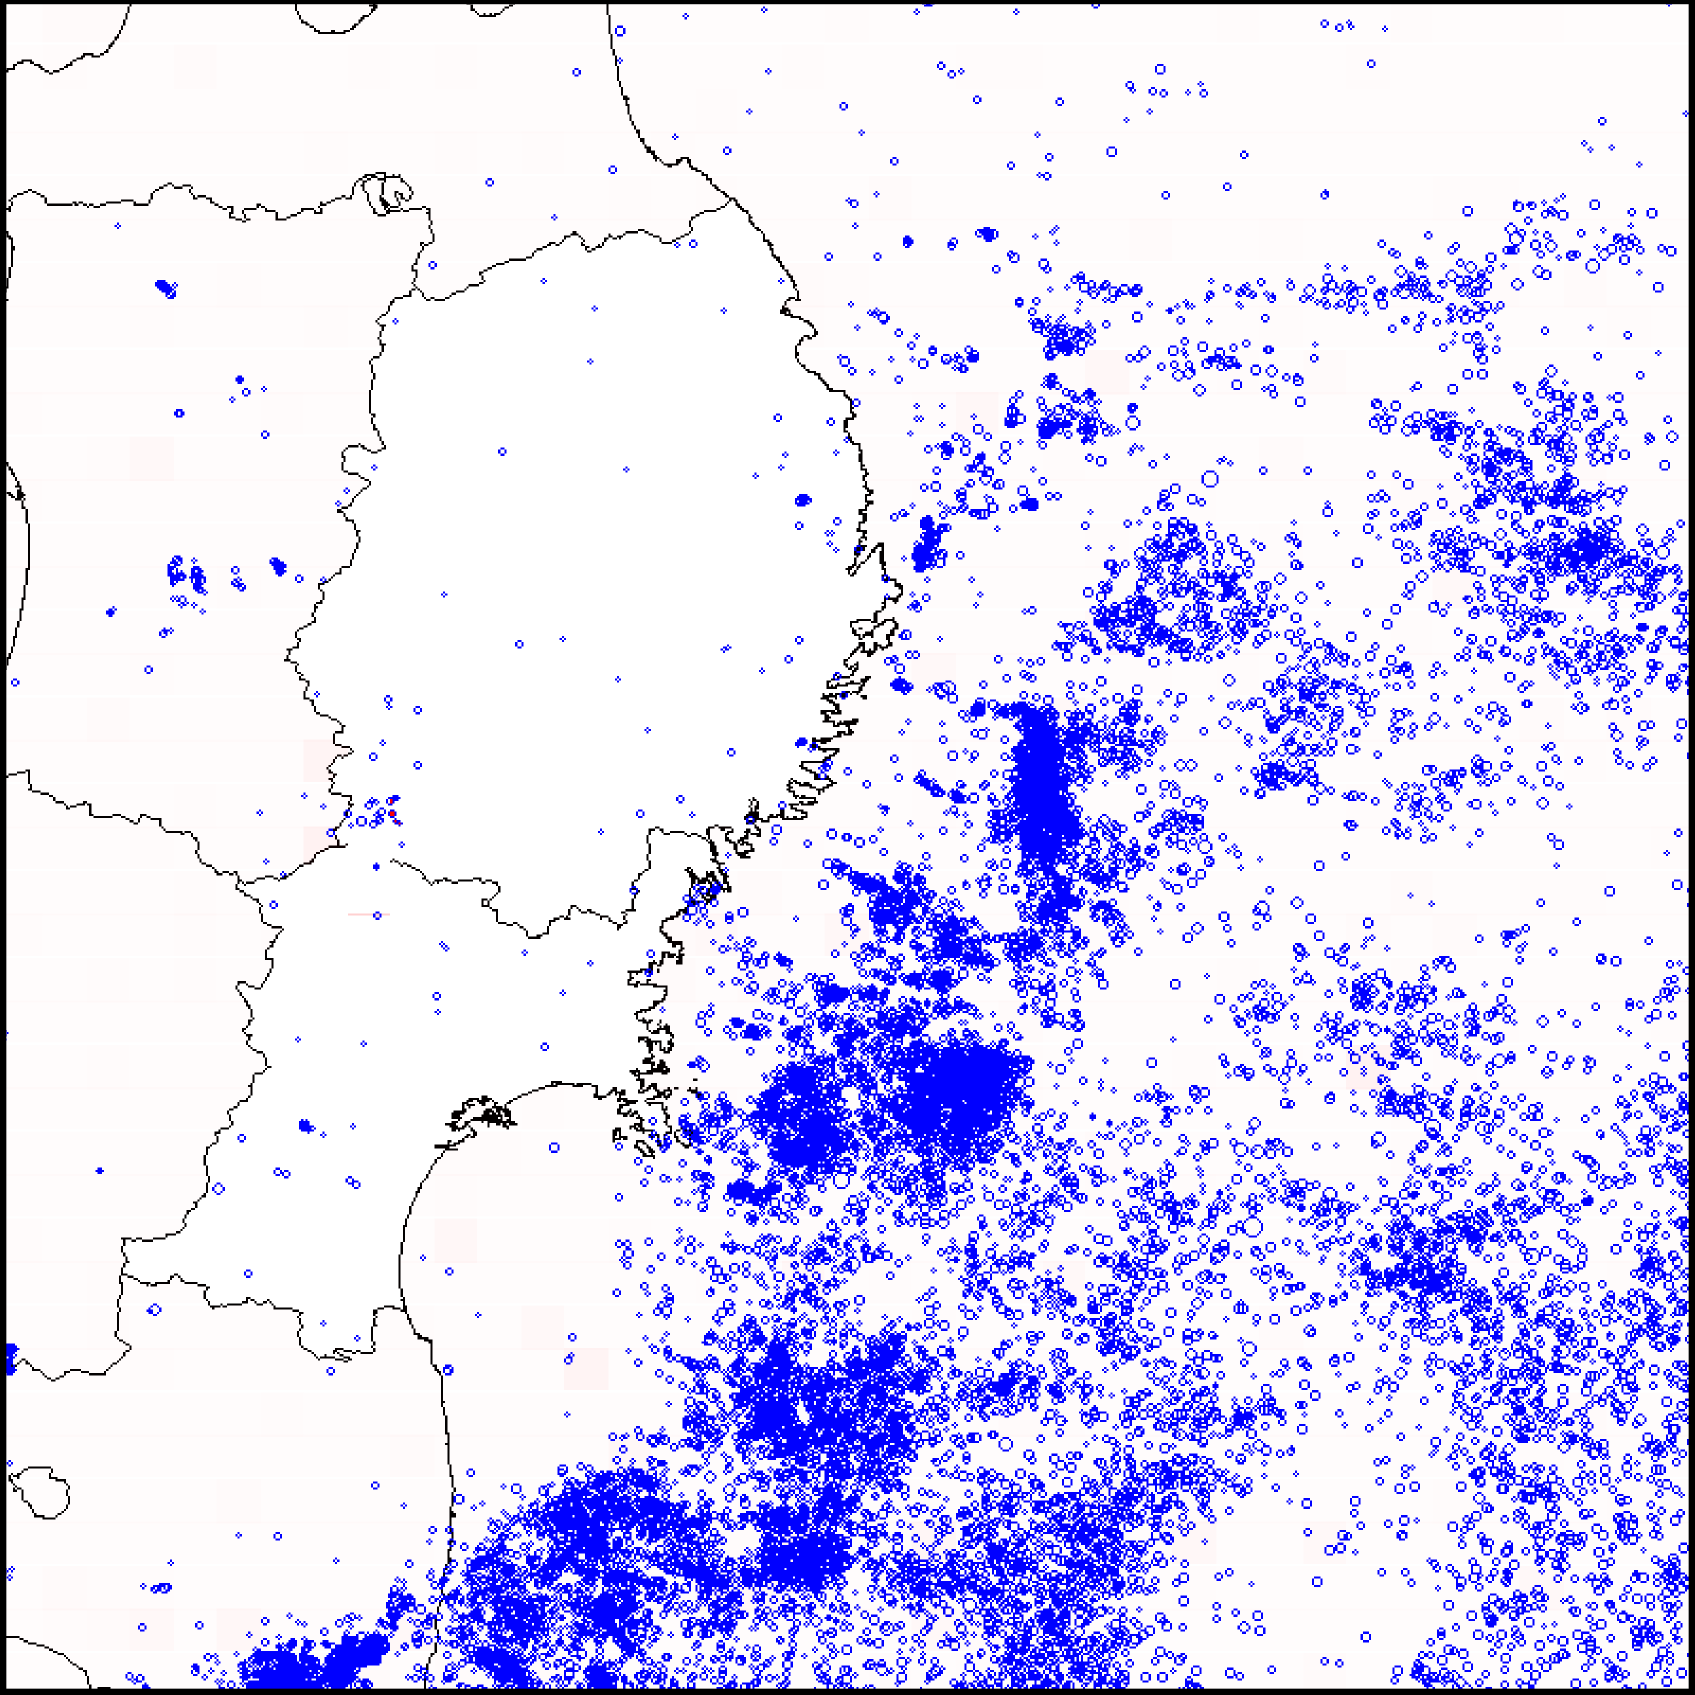
\includegraphics[width=.45\textwidth]{img/earthquakes2011.png}
\caption{Seismic Activity in Eastern Japan in 2011. Each dot
  shows one earthquake}
\label{GreatEastJapan}
\end{figure}

% Context of our work
In our previous work~\cite{ecta14}, we proposed a way to generate
earthquake risk models using a standard Genetic Algorithm (here called
the GAModel). The GAModel was shown to be competitive with the
Relative Intensity (RI) model. In this paper, the main goal is to observe the performance accomplished by the GAModel and a real-valued Genetic Algorithm (based on the GAModel, GA-BBOB) applied to 24 noise-free 40 dimensions BBOB benchmark functions. To achieve that, we first explore the number of individuals to be selected by the Tournament operator. Then we analyze the results of the GAModel and the results of the GA-BBOB to verify any relationship between applying the Tournament operator in the ``generating earthquake risk model'' function and applying tht Tournament operator in all the benchmark functions.


%TODO:
%change this when the scope is complete
These adaptions are described here and there. we do this and that here and there too. results and other stuff are here and there.